\section{Architectural Overview}\label{sec:arch}

%The basic architecture to develop a system like this, regarding the existing TUMOnline system where you can check if a student is enrolled or not, will consist of the following parts:
The basic architecture to develop the system outlined above will consist of the following parts:

\begin{itemize}
\item The smartphone, including a NFC chip as well as an internet connection to register with the service. An internet connection will only be needed once during initialisation of the system.
\item The door system, also including a NFC chip which can send and receive. A NFC reader would not suffice as it would be vulnerable to simple replay attacks. The door system also needs access to the internet or at least to an intranet in order to check if the student or the employee has access to the specific area and to get other information for realising security features like communication encryption. Therefore, some kind of computer is also needed, interacting with the NFC hardware as well as with the backend.
\item A back-end system, which will take care of key generation and storage in case of a public-key system.

\item The TUMOnline system, which has enrolment information about every student and can confirm the status of a person.
% since is in the possession of the enrollment information of every student.
\end{itemize} 
 
 
 The following figure gives a holistic overview of the basic architecture: \newline
 \begin{center}
	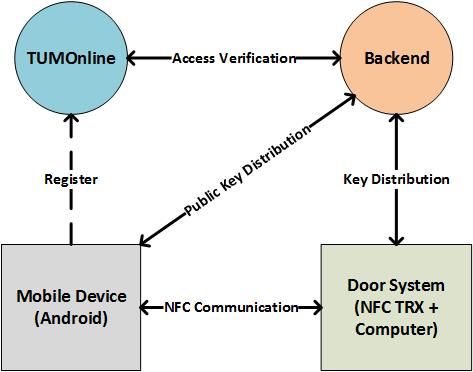
\includegraphics[scale=0.8]{basic_architecture.jpg}
\end{center}


\subsection{Registration with Back-end}
To initialise the system, the user has to contact the back-end system once for authentication.
The connection is planned to be secured by HTTPS.
The back-end system can check if the provided login data of the user is valid or not. 
In order to get this kind of information, TUMOnline services need to be contacted.
%For this purpose, the connection to the TUMOnline service is needed to get this kind of  information.
If the user has sent the right login combination, the back-end system will create a public key pair and will send the user his private key.
For this functionality, the back-end needs to work as a key storage and management system. It includes a simple yet secure database.
%Therefore, a key storage and management system, a simple database has to be implemented.


\subsection{Authentication between Smartphone and NFC Transceiver}
After the user has registered with the back-end system, he can communicate with the NFC reader.
A three-way handshake assures a secure connection between smartphone and NFC reader.
In order to verify the soundness of the procedure, in particular the authenticity of the communication partner, the NFC reader (i.e.~the system behind it) will fetch the public key of the user who wants to authenticate from the back-end system.
%As an initialisation, there is a three-way handshake to provide a secure connection where the NFC Reader and the system behind will fetch the public key of the specific user.
Furthermore, the door system will check if the user has access to the requested area.
It will finally unlock the door if all checks were positive.

